

\tikzset{every picture/.style={line width=0.75pt}} %set default line width to 0.75pt        

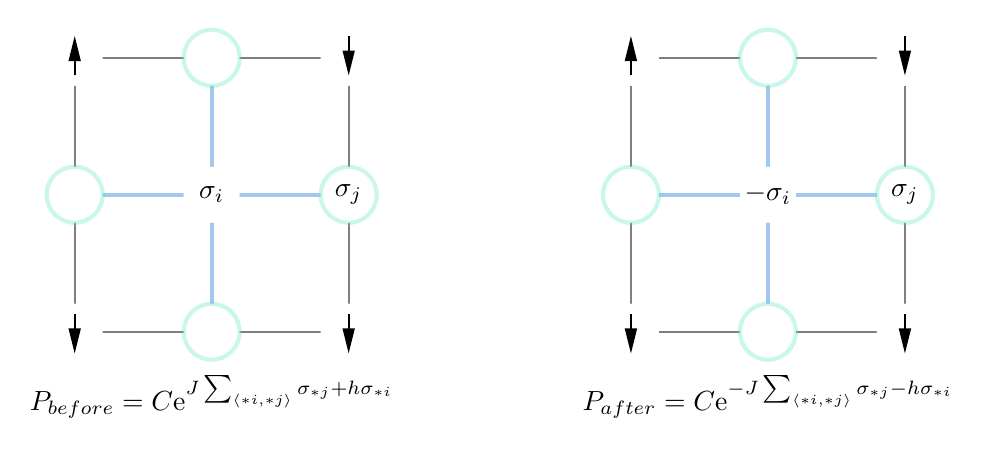
\begin{tikzpicture}[x=0.75pt,y=0.75pt,yscale=-1,xscale=1]
%uncomment if require: \path (0,300); %set diagram left start at 0, and has height of 300

%Straight Lines [id:da7900688343051199] 
\draw [color={rgb, 255:red, 74; green, 144; blue, 226 }  ,draw opacity=0.5 ][line width=1.5]    (102,134) -- (168,134) ;
%Straight Lines [id:da22968837564615008] 
\draw [color={rgb, 255:red, 74; green, 144; blue, 226 }  ,draw opacity=0.5 ][line width=1.5]    (168,68) -- (168,134) ;
%Straight Lines [id:da13157986418239975] 
\draw [color={rgb, 255:red, 74; green, 144; blue, 226 }  ,draw opacity=0.5 ][line width=1.5]    (168,134) -- (168,200) ;
%Straight Lines [id:da801148560717611] 
\draw [color={rgb, 255:red, 74; green, 144; blue, 226 }  ,draw opacity=0.5 ][line width=1.5]    (168,134) -- (234,134) ;
%Straight Lines [id:da6808408566351207] 
\draw [color={rgb, 255:red, 0; green, 0; blue, 0 }  ,draw opacity=0.5 ]   (234,68) -- (234,134) ;
%Straight Lines [id:da35890973732003917] 
\draw [color={rgb, 255:red, 0; green, 0; blue, 0 }  ,draw opacity=0.5 ]   (168,68) -- (234,68) ;
%Straight Lines [id:da7296987791011087] 
\draw [color={rgb, 255:red, 0; green, 0; blue, 0 }  ,draw opacity=0.5 ]   (168,200) -- (234,200) ;
%Straight Lines [id:da07996474880653448] 
\draw [color={rgb, 255:red, 0; green, 0; blue, 0 }  ,draw opacity=0.5 ]   (102,134) -- (102,200) ;
%Straight Lines [id:da27575937842607634] 
\draw [color={rgb, 255:red, 0; green, 0; blue, 0 }  ,draw opacity=0.5 ]   (234,134) -- (234,200) ;
%Straight Lines [id:da38042419134786254] 
\draw [color={rgb, 255:red, 0; green, 0; blue, 0 }  ,draw opacity=0.5 ]   (102,68) -- (102,134) ;
%Straight Lines [id:da504469642986344] 
\draw [color={rgb, 255:red, 0; green, 0; blue, 0 }  ,draw opacity=0.5 ]   (102,68) -- (168,68) ;
%Straight Lines [id:da16311920253073486] 
\draw [color={rgb, 255:red, 0; green, 0; blue, 0 }  ,draw opacity=0.5 ]   (102,200) -- (168,200) ;
%Shape: Circle [id:dp12660612618234834] 
\draw  [draw opacity=0][fill={rgb, 255:red, 255; green, 255; blue, 255 }  ,fill opacity=1 ] (154.5,134) .. controls (154.5,126.54) and (160.54,120.5) .. (168,120.5) .. controls (175.46,120.5) and (181.5,126.54) .. (181.5,134) .. controls (181.5,141.46) and (175.46,147.5) .. (168,147.5) .. controls (160.54,147.5) and (154.5,141.46) .. (154.5,134) -- cycle ;
%Shape: Circle [id:dp8272795300855829] 
\draw  [color={rgb, 255:red, 80; green, 227; blue, 194 }  ,draw opacity=0.3 ][fill={rgb, 255:red, 255; green, 255; blue, 255 }  ,fill opacity=1 ][line width=1.5]  (220.5,134) .. controls (220.5,126.54) and (226.54,120.5) .. (234,120.5) .. controls (241.46,120.5) and (247.5,126.54) .. (247.5,134) .. controls (247.5,141.46) and (241.46,147.5) .. (234,147.5) .. controls (226.54,147.5) and (220.5,141.46) .. (220.5,134) -- cycle ;
%Shape: Circle [id:dp37957345707032264] 
\draw  [color={rgb, 255:red, 80; green, 227; blue, 194 }  ,draw opacity=0.3 ][fill={rgb, 255:red, 255; green, 255; blue, 255 }  ,fill opacity=1 ][line width=1.5]  (154.5,68) .. controls (154.5,60.54) and (160.54,54.5) .. (168,54.5) .. controls (175.46,54.5) and (181.5,60.54) .. (181.5,68) .. controls (181.5,75.46) and (175.46,81.5) .. (168,81.5) .. controls (160.54,81.5) and (154.5,75.46) .. (154.5,68) -- cycle ;
%Shape: Circle [id:dp8415187405246769] 
\draw  [draw opacity=0][fill={rgb, 255:red, 255; green, 255; blue, 255 }  ,fill opacity=1 ] (220.5,68) .. controls (220.5,60.54) and (226.54,54.5) .. (234,54.5) .. controls (241.46,54.5) and (247.5,60.54) .. (247.5,68) .. controls (247.5,75.46) and (241.46,81.5) .. (234,81.5) .. controls (226.54,81.5) and (220.5,75.46) .. (220.5,68) -- cycle ;
%Shape: Circle [id:dp70137316267554] 
\draw  [draw opacity=0][fill={rgb, 255:red, 255; green, 255; blue, 255 }  ,fill opacity=1 ] (88.5,68) .. controls (88.5,60.54) and (94.54,54.5) .. (102,54.5) .. controls (109.46,54.5) and (115.5,60.54) .. (115.5,68) .. controls (115.5,75.46) and (109.46,81.5) .. (102,81.5) .. controls (94.54,81.5) and (88.5,75.46) .. (88.5,68) -- cycle ;
%Shape: Circle [id:dp36470096186038825] 
\draw  [draw opacity=0][fill={rgb, 255:red, 255; green, 255; blue, 255 }  ,fill opacity=1 ] (88.5,200) .. controls (88.5,192.54) and (94.54,186.5) .. (102,186.5) .. controls (109.46,186.5) and (115.5,192.54) .. (115.5,200) .. controls (115.5,207.46) and (109.46,213.5) .. (102,213.5) .. controls (94.54,213.5) and (88.5,207.46) .. (88.5,200) -- cycle ;
%Shape: Circle [id:dp7844046903427413] 
\draw  [color={rgb, 255:red, 80; green, 227; blue, 194 }  ,draw opacity=0.3 ][fill={rgb, 255:red, 255; green, 255; blue, 255 }  ,fill opacity=1 ][line width=1.5]  (154.5,200) .. controls (154.5,192.54) and (160.54,186.5) .. (168,186.5) .. controls (175.46,186.5) and (181.5,192.54) .. (181.5,200) .. controls (181.5,207.46) and (175.46,213.5) .. (168,213.5) .. controls (160.54,213.5) and (154.5,207.46) .. (154.5,200) -- cycle ;
%Shape: Circle [id:dp4884199260348432] 
\draw  [draw opacity=0][fill={rgb, 255:red, 255; green, 255; blue, 255 }  ,fill opacity=1 ] (220.5,200) .. controls (220.5,192.54) and (226.54,186.5) .. (234,186.5) .. controls (241.46,186.5) and (247.5,192.54) .. (247.5,200) .. controls (247.5,207.46) and (241.46,213.5) .. (234,213.5) .. controls (226.54,213.5) and (220.5,207.46) .. (220.5,200) -- cycle ;
%Shape: Circle [id:dp9817479765247512] 
\draw  [color={rgb, 255:red, 80; green, 227; blue, 194 }  ,draw opacity=0.3 ][fill={rgb, 255:red, 255; green, 255; blue, 255 }  ,fill opacity=1 ][line width=1.5]  (88.5,134) .. controls (88.5,126.54) and (94.54,120.5) .. (102,120.5) .. controls (109.46,120.5) and (115.5,126.54) .. (115.5,134) .. controls (115.5,141.46) and (109.46,147.5) .. (102,147.5) .. controls (94.54,147.5) and (88.5,141.46) .. (88.5,134) -- cycle ;
%Straight Lines [id:da040281492927668916] 
\draw    (102,76.5) -- (102,59.61) ;
\draw [shift={(102,57.61)}, rotate = 90] [fill={rgb, 255:red, 0; green, 0; blue, 0 }  ][line width=0.08]  [draw opacity=0] (12,-3) -- (0,0) -- (12,3) -- cycle    ;
%Straight Lines [id:da5030660845539701] 
\draw    (234,74.5) -- (234,57.61) ;
\draw [shift={(234,76.5)}, rotate = 270] [fill={rgb, 255:red, 0; green, 0; blue, 0 }  ][line width=0.08]  [draw opacity=0] (12,-3) -- (0,0) -- (12,3) -- cycle    ;
%Straight Lines [id:da1601353006246906] 
\draw    (102,208.39) -- (102,191.5) ;
\draw [shift={(102,210.39)}, rotate = 270] [fill={rgb, 255:red, 0; green, 0; blue, 0 }  ][line width=0.08]  [draw opacity=0] (12,-3) -- (0,0) -- (12,3) -- cycle    ;
%Straight Lines [id:da9308870465090386] 
\draw    (234,208.39) -- (234,191.5) ;
\draw [shift={(234,210.39)}, rotate = 270] [fill={rgb, 255:red, 0; green, 0; blue, 0 }  ][line width=0.08]  [draw opacity=0] (12,-3) -- (0,0) -- (12,3) -- cycle    ;
%Straight Lines [id:da9526311353771202] 
\draw [color={rgb, 255:red, 74; green, 144; blue, 226 }  ,draw opacity=0.5 ][line width=1.5]    (370,134) -- (436,134) ;
%Straight Lines [id:da7800672905673887] 
\draw [color={rgb, 255:red, 74; green, 144; blue, 226 }  ,draw opacity=0.5 ][line width=1.5]    (436,68) -- (436,134) ;
%Straight Lines [id:da40014270786563766] 
\draw [color={rgb, 255:red, 74; green, 144; blue, 226 }  ,draw opacity=0.5 ][line width=1.5]    (436,134) -- (436,200) ;
%Straight Lines [id:da18847794161043008] 
\draw [color={rgb, 255:red, 74; green, 144; blue, 226 }  ,draw opacity=0.5 ][line width=1.5]    (436,134) -- (502,134) ;
%Straight Lines [id:da18802111132727584] 
\draw [color={rgb, 255:red, 0; green, 0; blue, 0 }  ,draw opacity=0.5 ]   (502,68) -- (502,134) ;
%Straight Lines [id:da895120727488689] 
\draw [color={rgb, 255:red, 0; green, 0; blue, 0 }  ,draw opacity=0.5 ]   (436,68) -- (502,68) ;
%Straight Lines [id:da5273340139459683] 
\draw [color={rgb, 255:red, 0; green, 0; blue, 0 }  ,draw opacity=0.5 ]   (436,200) -- (502,200) ;
%Straight Lines [id:da4852932840110682] 
\draw [color={rgb, 255:red, 0; green, 0; blue, 0 }  ,draw opacity=0.5 ]   (370,134) -- (370,200) ;
%Straight Lines [id:da9929981254794022] 
\draw [color={rgb, 255:red, 0; green, 0; blue, 0 }  ,draw opacity=0.5 ]   (502,134) -- (502,200) ;
%Straight Lines [id:da11672432716461989] 
\draw [color={rgb, 255:red, 0; green, 0; blue, 0 }  ,draw opacity=0.5 ]   (370,68) -- (370,134) ;
%Straight Lines [id:da3301651139359456] 
\draw [color={rgb, 255:red, 0; green, 0; blue, 0 }  ,draw opacity=0.5 ]   (370,68) -- (436,68) ;
%Straight Lines [id:da0561955305873203] 
\draw [color={rgb, 255:red, 0; green, 0; blue, 0 }  ,draw opacity=0.5 ]   (370,200) -- (436,200) ;
%Shape: Circle [id:dp6834233943729904] 
\draw  [draw opacity=0][fill={rgb, 255:red, 255; green, 255; blue, 255 }  ,fill opacity=1 ] (422.5,134) .. controls (422.5,126.54) and (428.54,120.5) .. (436,120.5) .. controls (443.46,120.5) and (449.5,126.54) .. (449.5,134) .. controls (449.5,141.46) and (443.46,147.5) .. (436,147.5) .. controls (428.54,147.5) and (422.5,141.46) .. (422.5,134) -- cycle ;
%Shape: Circle [id:dp16739959004350213] 
\draw  [color={rgb, 255:red, 80; green, 227; blue, 194 }  ,draw opacity=0.3 ][fill={rgb, 255:red, 255; green, 255; blue, 255 }  ,fill opacity=1 ][line width=1.5]  (488.5,134) .. controls (488.5,126.54) and (494.54,120.5) .. (502,120.5) .. controls (509.46,120.5) and (515.5,126.54) .. (515.5,134) .. controls (515.5,141.46) and (509.46,147.5) .. (502,147.5) .. controls (494.54,147.5) and (488.5,141.46) .. (488.5,134) -- cycle ;
%Shape: Circle [id:dp32775829350034713] 
\draw  [color={rgb, 255:red, 80; green, 227; blue, 194 }  ,draw opacity=0.3 ][fill={rgb, 255:red, 255; green, 255; blue, 255 }  ,fill opacity=1 ][line width=1.5]  (422.5,68) .. controls (422.5,60.54) and (428.54,54.5) .. (436,54.5) .. controls (443.46,54.5) and (449.5,60.54) .. (449.5,68) .. controls (449.5,75.46) and (443.46,81.5) .. (436,81.5) .. controls (428.54,81.5) and (422.5,75.46) .. (422.5,68) -- cycle ;
%Shape: Circle [id:dp6123807309077447] 
\draw  [draw opacity=0][fill={rgb, 255:red, 255; green, 255; blue, 255 }  ,fill opacity=1 ] (488.5,68) .. controls (488.5,60.54) and (494.54,54.5) .. (502,54.5) .. controls (509.46,54.5) and (515.5,60.54) .. (515.5,68) .. controls (515.5,75.46) and (509.46,81.5) .. (502,81.5) .. controls (494.54,81.5) and (488.5,75.46) .. (488.5,68) -- cycle ;
%Shape: Circle [id:dp6112375647525954] 
\draw  [draw opacity=0][fill={rgb, 255:red, 255; green, 255; blue, 255 }  ,fill opacity=1 ] (356.5,68) .. controls (356.5,60.54) and (362.54,54.5) .. (370,54.5) .. controls (377.46,54.5) and (383.5,60.54) .. (383.5,68) .. controls (383.5,75.46) and (377.46,81.5) .. (370,81.5) .. controls (362.54,81.5) and (356.5,75.46) .. (356.5,68) -- cycle ;
%Shape: Circle [id:dp38443498445258095] 
\draw  [draw opacity=0][fill={rgb, 255:red, 255; green, 255; blue, 255 }  ,fill opacity=1 ] (356.5,200) .. controls (356.5,192.54) and (362.54,186.5) .. (370,186.5) .. controls (377.46,186.5) and (383.5,192.54) .. (383.5,200) .. controls (383.5,207.46) and (377.46,213.5) .. (370,213.5) .. controls (362.54,213.5) and (356.5,207.46) .. (356.5,200) -- cycle ;
%Shape: Circle [id:dp1659379994577168] 
\draw  [color={rgb, 255:red, 80; green, 227; blue, 194 }  ,draw opacity=0.3 ][fill={rgb, 255:red, 255; green, 255; blue, 255 }  ,fill opacity=1 ][line width=1.5]  (422.5,200) .. controls (422.5,192.54) and (428.54,186.5) .. (436,186.5) .. controls (443.46,186.5) and (449.5,192.54) .. (449.5,200) .. controls (449.5,207.46) and (443.46,213.5) .. (436,213.5) .. controls (428.54,213.5) and (422.5,207.46) .. (422.5,200) -- cycle ;
%Shape: Circle [id:dp08381955204398972] 
\draw  [draw opacity=0][fill={rgb, 255:red, 255; green, 255; blue, 255 }  ,fill opacity=1 ] (488.5,200) .. controls (488.5,192.54) and (494.54,186.5) .. (502,186.5) .. controls (509.46,186.5) and (515.5,192.54) .. (515.5,200) .. controls (515.5,207.46) and (509.46,213.5) .. (502,213.5) .. controls (494.54,213.5) and (488.5,207.46) .. (488.5,200) -- cycle ;
%Shape: Circle [id:dp8119392324387849] 
\draw  [color={rgb, 255:red, 80; green, 227; blue, 194 }  ,draw opacity=0.3 ][fill={rgb, 255:red, 255; green, 255; blue, 255 }  ,fill opacity=1 ][line width=1.5]  (356.5,134) .. controls (356.5,126.54) and (362.54,120.5) .. (370,120.5) .. controls (377.46,120.5) and (383.5,126.54) .. (383.5,134) .. controls (383.5,141.46) and (377.46,147.5) .. (370,147.5) .. controls (362.54,147.5) and (356.5,141.46) .. (356.5,134) -- cycle ;
%Straight Lines [id:da6166701649498854] 
\draw    (370,76.5) -- (370,59.61) ;
\draw [shift={(370,57.61)}, rotate = 90] [fill={rgb, 255:red, 0; green, 0; blue, 0 }  ][line width=0.08]  [draw opacity=0] (12,-3) -- (0,0) -- (12,3) -- cycle    ;
%Straight Lines [id:da2837693815237292] 
\draw    (502,74.5) -- (502,57.61) ;
\draw [shift={(502,76.5)}, rotate = 270] [fill={rgb, 255:red, 0; green, 0; blue, 0 }  ][line width=0.08]  [draw opacity=0] (12,-3) -- (0,0) -- (12,3) -- cycle    ;
%Straight Lines [id:da9872685865389901] 
\draw    (370,208.39) -- (370,191.5) ;
\draw [shift={(370,210.39)}, rotate = 270] [fill={rgb, 255:red, 0; green, 0; blue, 0 }  ][line width=0.08]  [draw opacity=0] (12,-3) -- (0,0) -- (12,3) -- cycle    ;
%Straight Lines [id:da08524866485503724] 
\draw    (502,208.39) -- (502,191.5) ;
\draw [shift={(502,210.39)}, rotate = 270] [fill={rgb, 255:red, 0; green, 0; blue, 0 }  ][line width=0.08]  [draw opacity=0] (12,-3) -- (0,0) -- (12,3) -- cycle    ;

% Text Node
\draw (168,219.5) node [anchor=north] [inner sep=0.75pt]   [align=left] { $\displaystyle P_\text{before} = C\mathrm{e}^{J \sum_{\langle \vb*{i}, \vb*{j} \rangle} \sigma_{\vb*{j}} + h \sigma_{\vb*{i}} } $};
% Text Node
\draw (168,134) node    {$\sigma _{\boldsymbol{i}}$};
% Text Node
\draw (234,134) node    {$\sigma _{\boldsymbol{j}}$};
% Text Node
\draw (436,219.5) node [anchor=north] [inner sep=0.75pt]   [align=left] { $\displaystyle P_\text{after} = C\mathrm{e}^{- J \sum_{\langle \vb*{i}, \vb*{j} \rangle} \sigma_{\vb*{j}} - h \sigma_{\vb*{i}} } $};
% Text Node
\draw (436,134) node    {$-\sigma _{\boldsymbol{i}}$};
% Text Node
\draw (502,134) node    {$\sigma _{\boldsymbol{j}}$};


\end{tikzpicture}
